\chapter{Ansatz}
Die inhaltliche Aufgabe der \textit{Textextraktion-18} war es alle Reden der 1. - 18. Wahlperiode zu extrahierten, hierbei sollten die vom \textit{Crawler} übergebenen XML-Dokumente extrahiert und in JSON Dateien ausgeben werden. Der \textit{Crawler} realisierte dies, durch die temporäre Persistierung der Plenarprotokolle als XML Dateien\cite{protokolle} und Übergabe als Parameter an die \textit{Textextraktion-18}.\\

\noindent Im Gegensatz zu den Plenarprotokollen der 19. Legislaturperiode liegen die Protokolle der 18. Legislaturperiode nicht in reinem XML Format vor (siehe \autoref{img:xml_begin_tags}), sondern es gibt am Anfang der XML Dateien die nötigsten XML Tags und das Protokoll selbst befindet sich in einem einzigen großen Textblock.
\begin{figure}[h]
	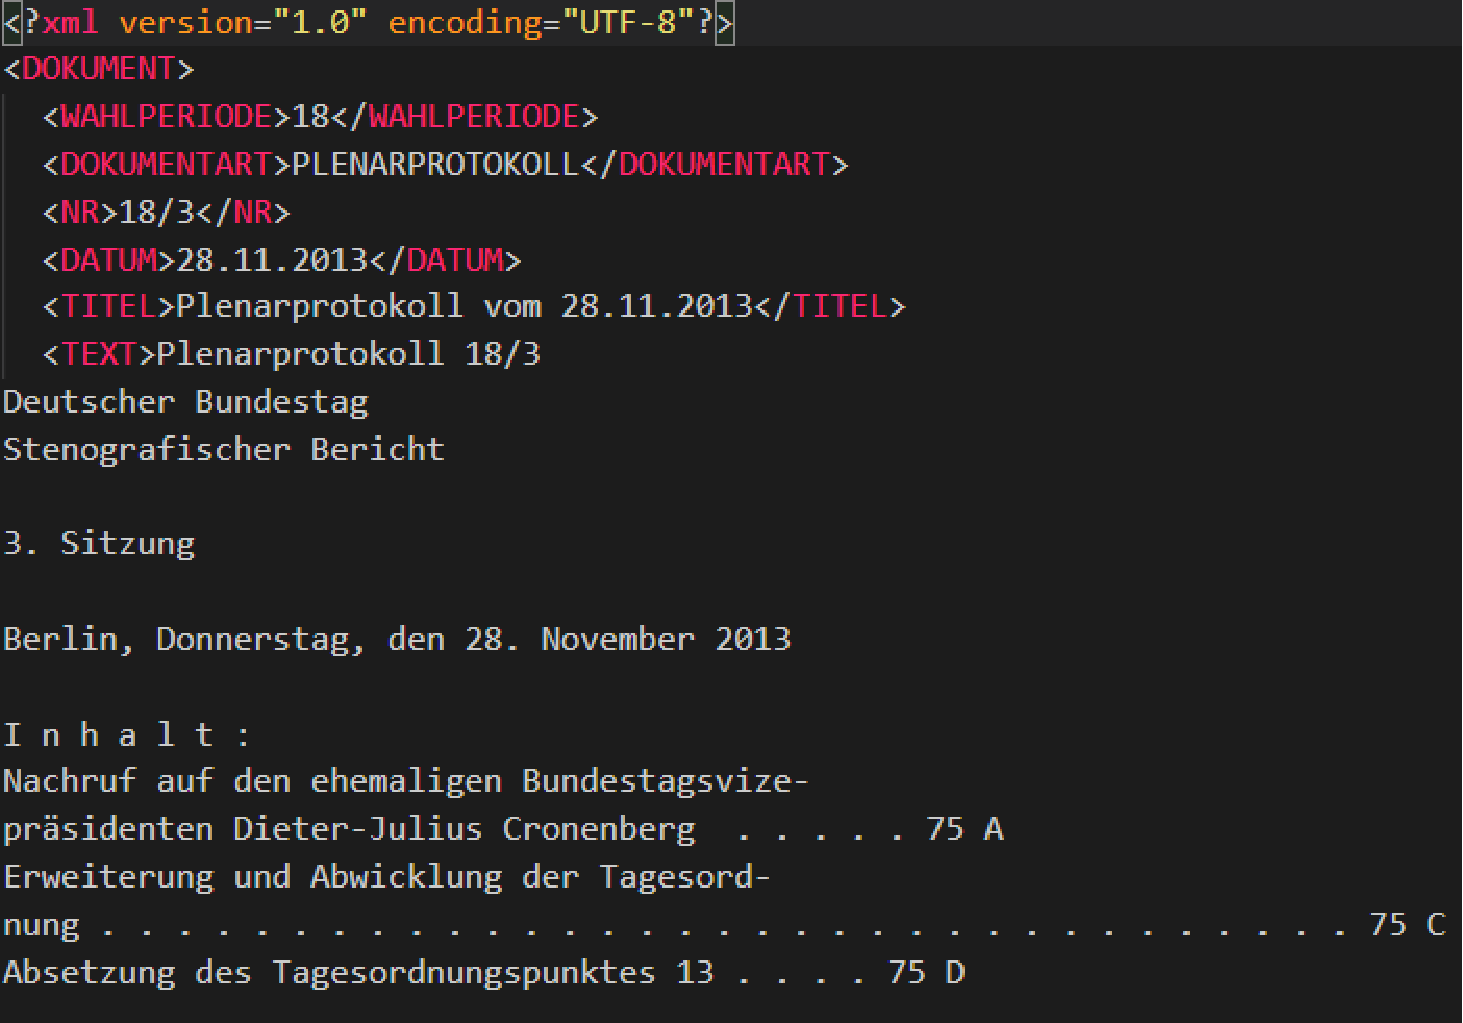
\includegraphics[width=\linewidth]{img/xml_begin_tags.pdf}
	\caption{18003.xml}
	\label{img:xml_begin_tags}
\end{figure}\\
Die Grundidee ist den Textblock semantisch und syntaktisch zu Untersuchen um einen Suchalgorithmus zu finden, welcher innerhalb des Textblockes:
\begin{multicols}{3}
	\begin{itemize}
		\item Titel der Rede
		\item Name des Sprechenden
		\item Zugehörigkeit
		\item Datum
		\item Rede
	\end{itemize}
\end{multicols}
zu einer Person findet und extrahiert.